\documentclass{article}
\usepackage[UTF8]{ctex}
\usepackage[T1]{fontenc}
\usepackage[utf8]{inputenc}
\usepackage{titlesec}
\usepackage[colorlinks, linkcolor = black]{hyperref}
\usepackage{float}
\usepackage{xcolor}
\usepackage{amsmath}
\usepackage{amssymb}
\usepackage{latexsym}
\usepackage{amsthm}
\usepackage{graphicx}
\usepackage{enumerate}
\usepackage{enumitem}
\usepackage{tikz}
\usetikzlibrary{positioning}
\usetikzlibrary[arrows, shapes, chains]

\setlist{
    leftmargin = .1\linewidth,
    % rightmargin = .1\linewidth,
    % label=\emph{\alph*}.
}

\titleformat{\section}[block]{\LARGE\scshape}{\arabic{section}}{1em}{}[]

\title{Homework 5}
\author{PB17000297 罗晏宸}
\date{March 29 2020}

\begin{document}
\maketitle

\section{Exercise 8.17}
解释下面给出的 Wumpus 世界中相邻方格的定义存在什么问题:
$$
    \forall x, y \quad \textit{Adjacent}([x, y], [x + 1, y]) \land \textit{Adjacent}([x, y], [x, y + 1])
$$

\paragraph{解}
这样的定义仅考虑了坐标轴正方向上的相邻,但实际上相邻关系是无向的(即对称的);另外定义没有考虑到世界边界的作用关系,可能会给出在实际问题中不存在的相邻关系。

一个更合理的定义是
\begin{equation*}
    \begin{aligned}
         & \forall 1 \leqslant x < 4, 1 \leqslant y < 4 \\ & \textit{Adjacent}([x, y], [x + 1, y]) \land \textit{Adjacent}([x + 1, y], [x, y]) \\ \land &\textit{Adjacent}([x, y], [x, y + 1]) \land \textit{Adjacent}([x, y + 1], [x, y])
    \end{aligned}
\end{equation*}

\section{Exercise 8.24}
用一个相容的词汇表(需要你自己定义)在一阶逻辑中表示下列语句:
\begin{enumerate}[label = \emph{\alph*}.]
    \item 某些学生在2001年春季学期上法语课
    \item 上法语课的每个学生都通过了考试
    \item 只有一个学生在2001年春季学期上希腊语课
    \item 希腊语课的最好成绩总是比法语课的最好成绩高
    \item 每个买保险的人都是聪明的
    \item 没有人会买昂贵的保险
    \item 有一个代理,他只卖保险给那些没有投保的人
    \item 镇上有一个理发师,他给所有不自己刮胡子的人刮胡子
    \item 在英国出生的人,如果其双亲都是英国公民或永久居住者,那么此人生来就是一个英国公民
    \item 在英国以外的地方出生的人,如果其双亲生来就是英国公民,那么此人血统上是一个英国公民
    \item 政治家可以一直愚弄某些人,也可以在某个时候愚弄所有人,但是他们无法一直愚弄所有的人
\end{enumerate}

\paragraph{解}
设计如下的词汇表:
\begin{itemize}
    \item $\textit{Student}(x)$表示$x$是学生
    \item $\textit{Select}(x, c, s)$表示学生$x$在$s$学期上$c$课
    \item $\textit{Pass}(x, c, s)$表示在$s$学期上$c$课的学生$x$通过了考试
    \item $\textit{Grade}(x, c, s)$表示在$s$学期上$c$课的学生$x$的成绩
    \item $\textit{Person}(x)$表示$x$是正常人
    \item $\textit{Smart}(x)$表示$x$是聪明的
    \item $\textit{Policy}(x)$表示$x$是保险
    \item $\textit{Expensive}(x)$表示$x$是昂贵的
    \item $\textit{Agent}(x)$表示$x$是代理
    \item $\textit{Insured}(x)$表示$x$已被投保
    \item $\textit{Buy}(x, y, g)$表示$x$向$y$购买了$g$
    \item $\textit{Sell}(x, y, g)$表示$x$把$g$卖给了$y$
    \item $\textit{Barber}(x)$表示$x$是理发师
    \item $\textit{Shave}(x, y)$表示$x$给$y$刮胡子
    \item $\textit{Born}(x, c)$表示$x$在国家$c$出生
    \item $\textit{Parent}(x, y)$表示$x$是$y$的双亲之一
    \item $\textit{Citizen}(x, c, b)$表示$x$基于$b$是国家$c$的公民
    \item $\textit{Resident}(x, c)$表示$x$是国家$c$的永久居住者
    \item $\textit{Politician}(x)$表示$x$是政治家
    \item $\textit{Fool}(x, y, t)$表示$x$在$t$时刻愚弄了$y$
\end{itemize}
给出上述语句的表示
\begin{enumerate}[label = \emph{\alph*}.]
    \item $\exists x \quad \textit{Student}(x) \land \textit{Select}(x, \textit{French}, \textit{2001Spring})$
    \item $\forall x,s \quad \textit{Student}(x) \land \textit{Select}(x, \textit{French}, s) \Rightarrow \textit{Pass}(x, \textit{French}, s)$
    \item $\forall x \quad \textit{Student}(x) \land \textit{Select}(x, \textit{Greek}, s) \land \big(\forall y \quad y \neq x \Rightarrow \lnot \textit{Select}(y, \textit{Greek}, \textit{2001Spring})\big)$
    \item $\forall s\ \exists x\ \forall y \quad \textit{Grade}(x, \textit{Greek}, s) > \textit{Grade}(y, French, s)$
    \item $\forall x,p,a \quad \textit{Person}(x) \land \textit{Policy}(p) \land \textit{Agent}(a) \land \textit{Buy}(x, a, p) \Rightarrow \textit{Smart}(x)$
    \item $\forall x,p,a \quad \textit{Person}(x) \land \textit{Policy}(p) \land \textit{Expensive}(p) \Rightarrow \lnot \textit{Buy}(x, a, p)$
    \item $\exists a \quad \textit{Agent}(a) \land \Big(\forall x, p \ \big(\textit{Policy}(p) \land \textit{Sell}(a, x, p)\big) \Rightarrow \big(\textit{Person}(x) \land \lnot \textit{Insured}(x)\big)\Big)$
    \item $\exists x \quad \textit{Barber}(x) \land \big(\forall y \ \textit{Person}(y) \land \lnot \textit{Shave}(y,y) \Rightarrow \textit{Shave}(x,y)\big)$
    \item $\forall x \quad \textit{Person}(x) \land \textit{Born}(x, \textit{UK}) \land \bigg(\forall y \ \textit{Parent}(y,x) \land \Big(\big(\exists b \ \textit{Citizen}(y, \textit{UK}, b)\big) \lor \textit{Resident}(y, \textit{UK})\Big)\bigg) \Rightarrow \textit{Citizen}(x, \textit{UK}, \textit{"Birth"})$
    \item $\forall x \quad \textit{Person}(x) \land \lnot \textit{Born}(x, \textit{UK}) \land \Big(\forall y \ \textit{Parent}(y,x) \land \big(\exists b \ \textit{Citizen}(y, \textit{UK}, b)\big)\Big) \Rightarrow \textit{Citizen}(x, \textit{UK}, \textit{"Descent"})$
    \item $\forall x \quad \textit{Politician}(x) \Rightarrow \big(\exists y \  \forall t \ \textit{Person}(y) \land \textit{Fool}(x, y, t)\big) \land \big(\exists t \ \forall y \ \textit{Person}(y) \land \textit{Fool}(x, y, t)\big) \land \lnot\big(\forall t \ \forall y \ \textit{Person}(y) \land \textit{Fool}(x, y, t)\big)$
\end{enumerate}

\section{Exercise 9.3}
假定知识库中只包括一条语句:$\exists x \textit{AsHighAs}(x,\, \textit{Everest})$,下列哪个语句是应用存在量词实例化以后的合法结果?
\begin{enumerate}[label = \emph{\alph*}.]
    \item $\textit{AsHighAs}(\textit{Everest},\, \textit{Everest})$
    \item $\textit{AsHighAs}(\textit{Kilimanjaro},\, \textit{Everest})$
    \item $\textit{AsHighAs}(\textit{Kilimanjaro},\, \textit{Everest}) \land \textit{AsHighAs}(\textit{BenNevis},\, \textit{Everest})$
\end{enumerate}

\paragraph{解}
语句b和c都是合法的结果,a不合法的原因是替换变元的应当是从未在知识库中出现过的常量符号,而不是已经出现过的\textit{Everest}。

\section{Exercise 9.4}
对于下列每对原子语句,如果存在,请给出最一般合一置换:
\begin{enumerate}[label = \emph{\alph*}.]
    \item $P(A,\, B,\, B),\ P(x,\, y,\, z)$
    \item $Q(y,\, G(A,\, B)),\ Q(G(x,\, x),\, y)$
    \item $\textit{Older}(\textit{Father}(y),\, y),\ \textit{Older}(\textit{Father}(x),\, \textit{John})$
    \item $\textit{Knows}(\textit{Father}(y),\, y),\ \textit{Knows}(x,\, x)$
\end{enumerate}

\paragraph{解}
可能的合一置换结果如下所示
\begin{enumerate}[label = \emph{\alph*}.]
    \item $\{A/x,\, B/y,\, B/z\}$
    \item 合一失败,$x$不能同时取$A$和$B$
    \item $\{y/\textit{John},\, x/\textit{John}\}$
    \item 合一失败,发生检验中$y$和$\textit{Father}(y)$无法合一
\end{enumerate}

\section{Exercise 9.6}
写出下列语句的逻辑表示,使得它们适用一般化假言推理规则:
\begin{enumerate}[label = \emph{\alph*}.]
    \item 马、奶牛和猪都是哺乳动物
    \item 一匹马的后代是马
    \item Bluebeard 是一匹马
    \item Bluebeard 是 Charlie 的家长
    \item 后代和家长是逆关系
    \item 每个哺乳动物都有一个家长
\end{enumerate}

\paragraph{解}
\begin{itemize}
    \item $\textit{Horse}(x)$表示$x$是马
    \item $\textit{Cow}(x)$表示$x$是奶牛
    \item $\textit{Pig}(x)$表示$x$是猪
    \item $\textit{Mammal}(x)$表示$x$是哺乳动物
    \item $\textit{Descendant}(x,y)$表示$x$是$y$的后代
    \item $\textit{Parent}(x,y)$表示$x$是$y$的家长
\end{itemize}
逻辑表示如下
\begin{enumerate}[label = \emph{\alph*}.]
    \item $\textit{Horse}(x) \Rightarrow \textit{Mammal}(x) \\ \textit{Cow}(x) \Rightarrow \textit{Mammal}(x) \\ \textit{Pig}(x) \Rightarrow \textit{Mammal}(x)$
    \item $\textit{Descendant}(x, y) \land \textit{Horse}(y) \Rightarrow \textit{Horse}(x)$
    \item $\textit{Horse}(\textit{Bluebeard})$
    \item $\textit{Parent}(\textit{Bluebeard}, \textit{Charlie})$
    \item $\textit{Descendant}(x, y) \Rightarrow \textit{Parent}(y, x) \\ \textit{Parent}(x, y) \Rightarrow \textit{Descendant}(y, x)$
    \item $\textit{Mammal}(x) \Rightarrow \textit{Parent}(\textit{Gen}(x), x)$,其中$\textit{Gen}(x)$是一个Skolem范式
\end{enumerate}

\section{Exercise 9.13}
本题中需要用到你在习题9.6中写出的语句,运用反向链接算法来回答问题
\subparagraph{a} 画出用穷举反向链接算法为查询$\exists h \textit{horse}(h)$生成的证明树,其中子句按照给定的顺序进行匹配
\subparagraph{b} 对于本邻域,你注意到了什么?
\subparagraph{c} 实际上从你的语句中得出了多少个$h$的解?
\subparagraph{d} 你是否可以想出一种方法找出所有的解?

\paragraph{解}
\subparagraph{a}
如图\ref{figure:1}所示。
\begin{figure}[h]
    \centering
    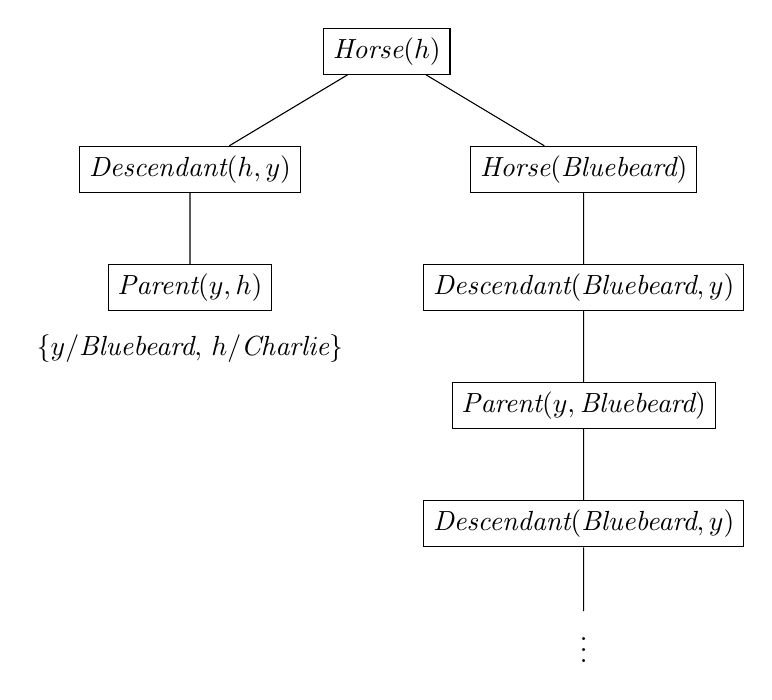
\begin{tikzpicture}[Node/.style = {rectangle, draw = black, text ragged}, sibling distance = 5cm]
        \node [Node] (1) {$\textit{Horse}(h)$}
        child {node [Node] (2) {$\textit{Descendant}(h,y)$}
                child {node [Node] (3) {$\textit{Parent}(y,h)$}}
            }
        child {node [Node] (4) {$\textit{Horse}(\textit{Bluebeard})$}
                child {node [Node] (6) {$\textit{Descendant}(\textit{Bluebeard},y)$}
                        child {node [Node] (7) {$\textit{Parent}(y, \textit{Bluebeard})$}
                                child {node [Node] (8) {$\textit{Descendant}(\textit{Bluebeard}, y)$}
                                        child {node [] (9) {$\vdots$}}
                                    }
                            }
                    }
            };
        \node [below = 0.5em of 3] (10) {$\{y/\textit{Bluebeard},\, h/\textit{Charlie}\}$};
    \end{tikzpicture}
    \caption{反向链接构造的证明树。其中$\textit{Parent}(y, \textit{Bluebeard})$和$\textit{Descendant}(\textit{Bluebeard}, y)$将会无限重复,无法到达树枝}
    \label{figure:1}
\end{figure}

\subparagraph{b}
注意到树中出现的无限延伸,这实际上是由于规则子句的顺序引起的,可以通过在规则$\textit{Descendant}(x, y) \land \textit{Horse}(y) \Rightarrow \textit{Horse}(x)$之前指定匹配顺序来得到解,但是如果要求穷举所有的解,那与子句顺序无关,循环一定会发生。

\subparagraph{c}
实际上得到了\textit{Bluebeard}和\textit{Charlie}两个解。

\subparagraph{d}
用堆栈维护子目标是否在搜索路径中出现过,当出现循环时,搁置该目标的证明,尝试证明其他所有分支,使用得到的解决方案作为该目标的解决方案,再继续对其证明以找到不同的解决方案,如果没有来自其他分支的解决方案使得该子目标成立,那么就认为其失败。
\end{document}